%% -*- mode: poly-noweb+R; ess-indent-level: 2; -*-

\chapter{Az \code{Rdev.xlam} bővítmény részletesebben}
\label{chap:6}


Ebbe a munkafüzetbe gyűjtöttem azokat a rutinokat, melyek csak a
fejlesztéshez szükségesek, 
lásd \aref{sec:3.1} szakaszt. Néhány olyan rutin is ide került, ami a
dokumentáció elkészítésében 
segített. Ez a fejezet a munkafüzet felépítését ismerteti.

\section{A \code{finalize} modul}\label{sec:6.1}

Itt vannak a számoló munkafüzet véglegesítésénél használt rutinok.
\begin{description}
\item[\code{FinalizeWb}] Először feloldjuk a lapvédelmet (\code{unprotectSheets}),
  majd elrejtjük az \code{R} kódot  (\code{HideRcodes}), a felhasználói cellák
  zárolását feloldjuk (\code{lockcells}), a bekapcsoljuk a lapvédelmet
  (\code{protectSheets}), végül elmentjük a munkafüzetet.  
\item[\code{HideRcodes}, \code{unHideRcodes}] Elrejtésnél végigmegyünk
  a munkalapokon. Ha az \code{isToHide} 
  függvény azt mondja egy munkalapról, hogy el kell rejteni, akkor
  elrejtjük és a \code{DEBUG/UNDEBUG} választéklista értékét \code{UNDEBUG}-ra
  állítjuk. Ellenkező esetben megnézzük, hogy az adott  munkalap
  nevei között szerepel-e az \code{R\_names}. Ha igen, akkor ennek az oszlopát
  is elrejtjük. Ez utóbbit az \code{Adatok} munkalapon használjuk.
  Visszaállításnál, csak az elrejtett munkalapokat és oszlopokat
  tesszük láthatóvá, nem változtatunk a \code{DEBUG/UNDEBUG} mező
  értékén. 
\item[\code{protectSheets}] Az aktív munkafüzet látható munkalapjainak védelmét
  bekapcsoljuk.  
\item[\code{unprotectSheets}] Az aktív munkafüzet valamennyi
  munkalapjának a védelmét kikapcsoljuk.  
\item[\code{lockcells}] Az aktív
  munkafüzet látható munkalapjain a használt tartomány celláinak
  \code{locked} tulajdonságát állítja be a cella színe alapján. Ha a cella
  színe (pontosabban \code{colorindexe}) azonos a
  \code{getCustomColor} értékkel, 
  akkor a felhasználó írhat a cellába, ellenkező esetben nem.  A
  rutin végén van egy rész, ami \code{checkbox} vezérlők használatát teszi
  lehetővé. Ha a  vezérlő \code{linkedcell} cellája ugyanazon a
  munkalapon van, akkor ez a cella sem lesz  zárolt. Ez a rész
  valószínűleg fölösleges.
\item[\code{isDebugDD(sh As Worksheet, dd As DropDown) As Boolean}] A
  \code{dd} \code{DropDown}-ról ellenőrzi,  hogy a 
  \code{DEBUG/UNDEBUG} választóról van-e szó.  
\item[\code{isToHide(name As String) As Boolean}] A \code{name}
  paraméterről ellenőrzi, hogy \code{R kód*} vagy  
  \code{*hidden*} alakú-e.  
\item[\code{getCustomColor}] Kikeresi a felhasználói mezők
  színét, pontosabban a \code{colorindex} tulajdonságát az \code{R kód} munkalap
  \code{colortable} tartományából.
\end{description}

\section{Az \code{insertform} modul}\label{sec:6.2}

%6.2. Az insertform modul
\subsection{\code{insert...} rutinok}

\begin{description}
\item[\code{insertAccessFrom}, \code{insertAccessSQLForm},
  \code{insertFileForm}, \code{insertDataLine}] Ezek a rutinok egy
  kaptafára mennek. A \code{Rdev.xlam} 
  munkafüzet \code{samples} munkalapján lévő mintákat  átmásoljuk a számoló
  munkafüzetbe, ha szükséges kis méretű gombokat illesztünk be  a
  megfelelő cellákba és ha kell a \code{R.xls} munkafüzetre mutató
  hivatkozást beállítjuk.  

  Az \code{insertDataLine} rutin kivételével egy
  elemet illesztünk be egyszerre az \code{activeCell} cellába (ez a kijelölés
  bal felső sarka). Az \code{insertDataLine} a kijelölés minden sorába 
  beilleszt egy \code{Data Line} elemet.
\item[\code{insertDropDown}] A kijelölt cellákba
  (pontosabban a kijelölés első oszlopának celláiba) beszúr  egy-egy
  \code{Drop Down} űrlapot. A választék listát pontos vesszővel elválasztott
  szövegként  a cella értékeként adhatjuk meg. Ha ez hiányzik,
  akkor egy felugró ablakban a lista hosszát kell megadni. Ez esetben
  utólag ki kell tölteni az \code{R kód} munkalap megfelelő tartományát. A
  tartomány fölé az \code{Adat} neve van beképletezve, ez a cellától balra
  álló mező értéke, mellé pedig a választott érték (Ide mutat az
  űrlap \code{linkedcell} tulajdonsága).  

  A rutin gondoskodik arról, hogy a
  \code{Drop Down} űrlap alatti cella képlete a választék lista  aktuális
  értékét tartalmazza és színe a tőle jobbra álló cella színével
  egyezzen meg. Így  véglegesítés után a felhasználó nem tudja
  elrontatni a képletezést.
\item[\code{insertCalcBtn (optional extra)}] Beszúr egy
  számolást indító gombot a kijelölt tartomány fölé. A gomb szövege
  \code{Számolás indítása} és makró hozzárendelését a \code{newRun} függvény
  számítja ki a gomb azonosítójából. Az eredmény alábbihoz hasonló
\begin{VBAframe}
Private Sub Btn1run() 
  runBtnClick Me.Shapes("Button 1") 
End Sub
\end{VBAframe}
 A
  \code{runBtnClick} az \code{R.xls} munkafüzet \code{Interface}
  moduljában van definiálva 
  és a \code{shape} alatti tartomány szövegét küldi el kiértékelésre az
  \code{R}-nek.  

  Ha a \code{insertCalcBtn} szubrutint nem üres \code{extra}
  paraméterrel hívjuk meg,
  %argumentumot is
  %megadjuk, 
   %  az eljárást,
  akkor az így megadott szöveg a
  \code{runBtnClick} sor végére kerül. Ha például
  \code{extra=",True"}, akkor a gomb makró-hozzárendelése 
\begin{VBAframe}
Private Sub Btn1run() 
  runBtnClick Me.Shapes("Button 1"), True 
End Sub
\end{VBAframe}
alakúra változik. Az első változat aszinkron módon hajtja végre a kódot, míg
a második szinkron módon.  Az \code{extra} paramétert a dokumentáció
készítése közben használtam.
\end{description}

\subsection{Segéd rutinok}
\begin{description}
\item[\code{formcopy(cell As Range)}] Ezt az eljárást a
  \code{insert...form} nevű rutinokból hívjuk, miután 
  az \code{Rdev.xlam} munkafüzet samples munkalapján a megfelelő részt
  másolásra kijelöltük. 
  A \code{cell} tartományba illesztjük a másolandó rész formuláit és
  formázását. A végén a beillesztett részt kijelöljük a \code{select}
  metódussal és a színeket a \code{setcolors} rutinnal a 
  számoló munkafüzettel összhangba hozzuk. 

\item[\code{insertSelectBtn(vbcs as Collection, c As Range, which As String, Optional exarg = "")}]
A \code{c} cella bal felső sarkába illeszt egy kis méretű gombot a
\code{smallBtnAt} eljárás segítségével. A gombhoz a \code{which}
paraméter alapján megfelelő makrót rendel. A \code{newSelect} 
szubrutinnal kiszámolt makrót feljegyezzük a \code{vbcs
  collection}ban. Az egyes típusok esetén a következő szubrutinok lehetségesek
\begin{VBAframe}
Private Sub File7Click()
  selectFile Me.Shapes("Button 7").TopLeftCell, "R,*.R"
End Sub
Private Sub mappa6Click()
  selectmappa Me.Shapes("Button 6").TopLeftCell
End Sub
Private Sub SQL5Click()
  selectSQL Me.Shapes("Button 5").TopLeftCell, 4, 2
End Sub
Private Sub TBL4Click()
  selectTBL Me.Shapes("Button 4").TopLeftCell
End Sub
Private Sub MDB3Click()
  selectMDB Me.Shapes("Button 3").TopLeftCell
End Sub
\end{VBAframe}
A \code{select...} szubrutinok a \code{R.xls} munkafüzet
\code{selectfuns} moduljában vannak definiálva. 
\item[\code{smallBtnAt (c as range)}] A \code{c} tartomány bal felső sarkába
elhelyez egy kis méretű gombot. A gomb szövegét törli. A méreteket a
modul elején definiált konstansok adják 
\begin{VBAframe} 
Const smallwd = 13 ' szélesség
Const smallht = 5  ' magasság
Const smallpd = 2  ' távolság a tartomány szélétől, padding
\end{VBAframe}
Túl kicsi cella esetén figyelmeztetést ad.
\item[\code{newRun}] Összerakja a \code{run} gombok makrójának szövegét.
\item[\code{newSelect}] Összerakja a \code{select} gombok makrójának szövegét.
\item[\code{setcolor(r As Range, Optional color)}] Ez a rutin színezi
  át a beillesztett elemeket a számoló munkalap aktuális
  színeire. Ehhez egyrészt \code{R kód} munkalap \code{colortable} nevű 
  tartományát használja, másrészt a \code{Rdev.xlam} bővítmény ugyanilyen
  nevű tartományát. 

  Ha a \code{color} paraméter meg van adva, akkor a számoló munkafüzet
  \code{color} nevű színe lesz az új elem háttérszíne. 
\item[\code{newListFillRange}] Kiszámolja, mi legyen az új
  \code{Drop down} választó űrlap \code{Listfillrange} tulajdonsága. Innen veszi
  az űrlap a lehetséges értékeket. Az eljárás a következő: az \code{R kód}
  munkalap \code{\$A} oszlopának aljáról indulunk és addig megyünk,
  amíg nem üres mezőt találunk. 
  Ez alá rakjuk a szükséges méretű tartományt.
\end{description}


\section{Az \code{insertR} modul}\label{sec:6.3}
Itt vannak az \code{R kódlap}ok kezelésére szolgáló rutinok.

\begin{description}
\item[\code{insertRfile}] Ennek a rutinnak a feladata az beszúrandó
  \code{R} file, fileok elérési útjának meghatározása. Ehhez
  megjelenít egy file választó dialógot, majd minden egyes
  kiválasztott file-ra végrehajtja a \code{insertRcode} szubrutint.
\item[\code{insertRcode(Rfile, wb As Workbook)}] A megadott
  \code{Rfile} tartalmát megpróbálja beszúrni a \code{wb}
  munkafüzetbe. Ha már 
  létezik a megadott \code{R kódlap}, akkor rákérdez, hogy 
  frissítse-e a (a \code{sheetUpdate} eljárással) kódlap tartalmát. Ha
  nem létezik ilyen nevű kódlap, akkor létrehoz egy újat és abba
  beilleszti a file tartalmát az \code{insertRtoSheet} eljárással. 
\item[\code{insertRtoSheet(wb As Workbook, ws As Worksheet, Rfile)}]
  Először a \code{sheetUpdate} szubrutin segítségével feltölti a
  \code{ws} munkalapot a \code{Rfile} tartalmával, majd a munkalapra
  beilleszti a \code{Workheet\_Change} esemény kezelő eljárást. Ezt
  arra használjuk, hogy ha a kódlap 
  tartalma változik, akkor annak időpontját feljegyezhessük a
  munkalapon. A beillesztett kód
\begin{VBAframe}
Private Sub Worksheet_Change(ByVal Target As Range)
  If Target.Row > 1 Then
    Me.Cells(1, 1).Value = _
      "'" & "## sheet last modified: " & CStr(VBA.Date + VBA.Time)
  End If
End Sub
\end{VBAframe}
\item[\code{sheetUpdate}] A munkalap harmadik sora után beilleszti a
  file tartalmát, majd az első három sorba beszúrja a \code{fileinfo} részt
  az \code{insertRfileInfo} eljárással. 
\item[\code{insertRfileInfo}] A \code{fileinfo} a munkalap utolsó
  módosításának időpontja, a forrás teljes 
  elérési útja, és a forrás utolsó módosításának időpontja. Lásd
  \aref{fig:1.4} ábrán. Ennek beillesztése után a munkalap betű
  típusát \code{Lucida console}-ra állítjuk 10-es betűmérettel. Ez 
  egy \code{monospace} betűtípus. Végül beállítjuk az első oszlop
  szélességét az \code{autofit} metódus segítségével.
\item[\code{updateAllRsources}] Végigmegy az aktív munkafüzet
  munkalapjain, és az \code{R kódlap}okat frissíti. Ha munkalap
  tartalma változott, rákérdez arra, hogy tényleg frissítsen-e. Egy
  munkalapot akkor tekintünk \code{R kódlap}nak, ha neve \code{R
    kód(<filenév>)} alakú. A frissítés a \code{sheetUpdate}
  szubrutinnal történik. 
\item[\code{saveAllRsources}] Végigmegy az aktív munkafüzet
  munkalapjain, és az \code{R kódlap}okat menti 
  a \code{sheetSave} eljárással. Ha ezzel információt veszhetne el,
  akkor a felhasználó dönthet 
  a mentésről.
\item[\code{sheetSave(sh As Worksheet, Rfile)}] Kiírja az \code{sh}
  munkalap első oszlopának a tartalmát (az első három sor nélkül) a
  megadott \code{Rfile} állományba és frissíti a \code{fileInfo} mezőket. 
\item[\code{getfinfo,rmprefix}] Ezek segédfüggvények a \code{fileInfo} mezők
  kezeléséhez. 
\end{description}


\section{Az \code{insertSkeleton} modul}\label{sec:6.4}

Itt van az a rutin, ami a \code{Calc.xlt} template alapján létrehoz
egy új számoló munkafüzetet. A modul többi része a munkafüzetek
színezésével foglalkozik. Itt színekből álló \code{collection}okkal
dolgozunk, ahol az elemek kulcs-a a helyettesítendő szín \code{RGB} kódja,
míg értéke az új szín \code{RGB} kódja. Ezt nevezhetnénk akár színkulcsnak is.

\begin{description}
\item[\code{newSkeleton(Optional fname = False)}] Létrehozunk egy új
  munkafüzetet a \code{Calc.xlt} template alapján, beállítjuk a
  \code{R.xls} munkafüzetre mutató hivatkozást majd elmentjük a 
  munkafüzetet. Ha a \code{fname} argumentum nem \code{False}, akkor ez
  lesz a mentett munkafüzet neve, ellenkező esetben a felhasználó
  választ a \code{EXCEL} \code{saveAsFilename} dialógjával. 
  Pillanatnyilag az \code{xls} formátumot erőltetjük mentéskor. Ha ezt
  meg akarjuk változtatni, 
  akkor a modul elején található \code{wbFormat} konstans értékét kell
  átállítani. Eredetileg ez a rutin másolta át a \code{Thisworkbook} modul
  \code{checkRefToR} szubrutinját az 
  újonnan létrehozott számoló munkafüzetbe. Ennek az az előnye, hogy
  elegendő egy helyen a \code{Rdev.xlam} munkafüzetben javítani a
  kódot. Azonban, az \code{EXCEL} korábbi (\code{XP})  változata ettől
  rendszeresen összeomlott. Kicsit böngészve a netet arra jutottam, hogy
  ezt a hibát mások is tapasztalták és nem tudom javítani. Ezért került
  a \code{checkRefToR} a \code{Calc.xlt} sablonba is. Így azonban a
  javításokat mindkét helyen át kell vezetni. 
\item[\code{repaintWb}] Ez a szubrutin a kijelölt tartomány első
  oszlopát régi színként, második oszlopát a hozzá tartozó új színként
  értelmezi. Az így összeállított színkulcsot alkalmazza a 
  kijelölés munkafüzetére a \code{changeColorsWb} rutin segítségével. 
\item[\code{changeColorsWb(wb As Workbook, colors As Collection)}] A
  \code{wb} munkafüzet minden egyes munkalapjának használt
  tartományára alkalmazza a \code{changeColors} rutint. 
\item[\code{changeColors(r As Range, colors As Collection)}] Az
  \code{r} tartományt színezi át a colors 
  színkulcs segítségével.
\item[\code{insertUsedColors}] A kijelölt tartomány celláit az őt
  tartalmazó munkafüzet színeivel tölti ki. 
\item[\code{usedColors(wb As Workbook) As Collection}] A \code{wb}
  munkafüzetből kigyűjti a használt színeket.
\end{description}

\section{Az \code{insertVB} modul}\label{sec:6.5}

Ez a modul (az \code{rDir} függvény kivételével) programozottan próbál
hozzáférni a \code{EXCEL} \code{VBA projekt} objektummodelljéhez. Csak akkor
működik, ha a
\begin{verbatim}
File->Beállítások->Adatvédelmi központ->Makróbeállítások
\end{verbatim}
lapon a ,,A VBA projekt objektmodelljéhez való hozzáférés megbízható''
címkéjű checkboxot kipipáljuk. 
\begin{description}
\item[\code{VBAaccess}] Ez a függvény ellenőrzi, a \code{VBA projekt
    objektummodell}hez való hozzáférés lehetőségét. Ha nem
  engedélyezett tájékoztatja a felhasználót a teendőkről. 
\item[\code{insertVB(ws as worksheet, code As String, procname)}] 
  Beilleszti a \code{code}
  sztringet a  
  \code{ws} munkalap \code{CodeModule}jába. A \code{procname} a
  \code{code}-ban megadott eljárás 
  neve. Csak akkor  illesztjük be a kódot, ha nincs \code{procname}
  nevű eljárás vagy függvény. 
  
  Ez a rutin sok fejtörést okozott, mert sokáig nem működött
  megbízhatóan. A megoldás kulcsa a a munkalap 
  \code{CodeModule}jának megtalálása a \code{getCM} függvénnyel. Ha az
  \code{R kódlap}ok beszúrása során nem  jön létre a \code{Worksheet\_Change}
  makró, akkor itt kell keresni az okát. 
\item[\code{insertVBcoll(vbcs as collection)}] Erre a rutinra azért
  van szükség, mert az \code{EXCEL} \code{XP} változata összeomlott, ha több
  kódrészletet szúrtam be egymás után. A \code{vbcs} egy \code{VBcode} 
  típusú elemekből álló \code{collection}. Minden elemnek három
  tulajdonsága van: \code{id}, \code{code}, \code{ws} ami egy munkalap
  objektum. Először megkeresi, a \code{CodeModule}-t, amibe a kódot be 
  kell illeszteni. Ezután összefűzi azokat a kódrészleteket, amelyek
  \code{id}je még nincs definiálva a \code{CodeModule}ban. Végül
  beszúrja az így kapott szöveget. 

\item[\code{nameExists(cl As Object, name) As Boolean}] Ellenőrzi,
  hogy a \code{cl}
  \code{collection} jellegű objektumban létezik-e
  olyan elem, aminek \code{name} tulajdonsága azonos a \code{name}
  paraméterrel. Tipikus használata: 
\begin{VBAframe}
If Not (nameExists(Wb.VBProject.References, "R")) Then
  Wb.VBProject.References.AddFromFile _
    ThisWorkbook.VBProject.References.Item("R").FullPath
End If
\end{VBAframe}
\item[\code{procString(cmodule as CodeModule, procname) As String}]
  Visszaadja a \code{cmodule} modul \code{procname} nevű eljárásának szövegét.
\item[\code{procExists(cmodule as CodeModule, procname) As Boolean}]
  \code{Igaz} értéket ad vissza, ha a \code{cmodule}
  \code{CodeModule}ban létezik \code{procname} nevű eljárás, vagy függvény. 
\item[\code{rDir}] Az \code{appdata} környezeti változóból kiszámolja
  a \code{R.xls} munkafüzet könyvtárát. 
\item[\code{SetReftoRxls (wb as Workbook)}] A \code{wb} munkafüzet
  hivatkozásai közé felvesszük a \code{R.xls} 
  munkafüzetet, ha az nincs ott.
\item[\code{getCM(ws As Worksheet) As CodeModule}] A \code{ws}
  \code{Worksheet}hez tartozó \code{CodeModule}t keresi meg.

Amikor programozottan hozunk létre egy új munkalapot, akkor
közvetlenül a létrehozás után a hozzá tartozó \code{CodeModule} elérésére 
\begin{VBAframe}
wb.VBProject.VBComponents ("<worksheet name>")
\end{VBAframe}
nem alkalmas. Ezért alkalmazza a rutin a körülményesebb
\begin{VBAframe}
For Each vc In wb.VBProject.VBComponents
  If cname = vc.Properties("Name") Then Exit For
    Set vc = Nothing
Next
\end{VBAframe}
megoldást.
\end{description}

\section{Egyebek}\label{sec:6.6}

\subsubsection{A \code{Thisworkbook} modul}

A modul legnagyobb része az \code{EXCEL} különböző menüinek beállítása az
\code{addMenu} rutinnal. A \code{removeMenu (cb, mcaption)} rutin a
\code{cb} \code{commandBar} \code{mcaption} nevű menüjét törli. Ennek 
felhasználásával a \code{removemenus} az összes munkafüzet által
telepített menüt törli. 

Az \code{addMenu} rutinban a menük telepítése
előtt a korábbi változatot töröljük. Ezt a rutint a 
munkalap betöltésekor és a bővítmény telepítésekor futtatjuk le. A
rutin elején használjuk 
a \code{checkRefToR} függvényt. A visszatérési érték \code{IGAZ}, ha a
megfelelő \code{R.xls} munkafüzetet 
sikerült megnyitni, vagy eleve nyitva volt és \code{HAMIS}
egyébként. Ha van ugyan megnyitva 
\code{R.xls} munkafüzet, de elérési útja nem az elvárt, akkor
megpróbáljuk a rá mutató hivatkozást törölni és a jó hivatkozást
beállítani.


A menük törlését vagy a \code{Workbook\_Close} vagy a
\code{Workbook\_AddInUninstall} rutinból indítjuk el. A munkafüzet bezárásakor csak akkor töröljük a menüket, ha a \code{Rdev.xlam} munkafüzet
nincs bővítményként telepítve. 

\subsubsection{A \code{capturewnd} modul}
A \code{capturewnd} szubrutin a megadott ablak (\code{hwnd}) képét
\code{bmp} formátumban menti a megadott 
fileba (\code{fname}). Ennek a dokumentációnak a képernyőképei
készültek a segítségével. 

\subsubsection{A \code{saveVBE} modul}

Egyetlen szubrutint definiál \code{saveAllVBE} névvel. A felhasználó
által kiválasztott könyvtárba 
menti a megnyitott munkafüzetek \code{Visual Basic} kódját. Mindegyik
\code{VBAProject}-et a nevével megegyező alkönyvtárba próbál
menteni. Mentés előtt rákérdez, hogy az adott projektet 
valóban menteni szeretnénk-e. Az egyes \code{VB} komponensek mentése
az export metódussal történik.

\subsubsection{A \code{RIBBON} modul}

Egyetlen szubrutint tartalmaz, \code{menufunction} névvel. Ez a
\code{RIBBON} felületen definiált gombok makrója, a gomb azonosítója
alapján a megfelelő eljárást hívja meg.

Azért, hogy a bővítményt \code{EXCEL} XP-be is be lehessen tölteni ez a modul
csak akkor fordítódik le, ha \code{VBA7} konstans definiálva van. Ez
biztosan teljesül \code{OFFICE 2010} és \code{2013} esetén. 
Az \code{OFFICE 2003} ill. \code{OFFICE 2007} változatokkal nincs tapasztalatom.

\subsubsection{A samples munkalap (\ref{fig:6.1} ábra)}

Ezen a munkalapon vannak az \code{Access Form} és \code{ACCESS + SQL}
valamint a \code{Data Line} elemek mintái. Innen másoljuk át őket a megfelelő
menüparancs hatására. 
%6.1. ábra. A samples munkalap képe
\begin{figure}[h]
  \centering
  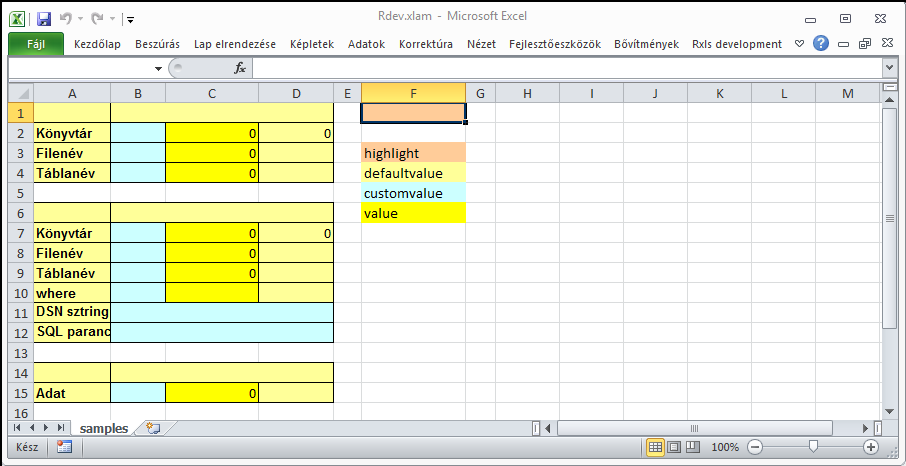
\includegraphics{images/samples}
  \caption{A samples munkalap képe}
  \label{fig:6.1}
\end{figure}

\begin{Rnw}
<<echo=FALSE,results="hide">>=
withObj(THISXL,{
  .[["height"]]<-350
  setRibbon(.,hide=TRUE)
  withObj(.$workbooks("Rdev.xlam"),{
    .[["isaddin"]]<-FALSE
    .$names("path")$referstorange()$select()
    capturewnd("samples.bmp")
    .[["isaddin"]]<-TRUE
  })
})

@
\end{Rnw}

\endinput


%%% Local Variables: 
%%% mode: latex
%%% TeX-master: "Rxls"
%%% End: 
